\documentclass[10pt]{article}

\usepackage{siunitx}
\usepackage{amsmath}
\usepackage{amsfonts}
\usepackage{booktabs}
\usepackage[margin=0.75in]{geometry}
\usepackage{graphicx}
\usepackage{mhchem}

\renewcommand{\vec}{\mathbf}
\newcommand{\R}{\mathbb{R}}


\begin{document}
  \begin{tabular}{l}
    Box Num. 33 \\
    Problem Set 33 \\
    \today
  \end{tabular}

  \begin{enumerate}
    \item \begin{enumerate}
        \item The stable isotopes of \ce{^{76} Ge} are \ce{^{70} Ge}, \ce{^{72} Ge}, \ce{^{73} Ge}, \ce{^{74} Ge}, and \ce{^{76} Ge} itself.

        The stable isotones of \ce{^{76} Ge} are \ce{^{80} Kr}, \ce{^{79} Br}, \ce{^{78} Se}, and \ce{^{76} Ge}.

        The stable isobars of \ce{^{76} Ge} are \ce{^{76} Se} and \ce{^{76} Ge}.

        \item The mass defect of \ce{^3 H} is 0.008557u, which corresponds to a binding energy of $\SI{7.97}{\mega\electronvolt}$.

        For \ce{^3 He}, the mass defect is 0.00718853u, corresponding to a binding energy of $\SI{6.696}{\mega\electronvolt}$. The decrease in binding energy is due to the repulsion between the two protons in the \ce{^3 He} nucleus.

        \item The mass defect in going from \ce{^{17} O} to \ce{^{16} O} + \ce{n} is 0.00305938u, which corresponds to an energy of $\SI{2.85}{\mega\electronvolt}$.

        \item The mass defect going from \ce{^{40} Ca} to \ce{^{39} K} + \ce{p} is 0.00839216u, which corresponds to an energy of $\SI{7.187}{\mega\electronvolt}$.
    \end{enumerate}

    \item In Rutherford scattering, the closest approach of this incident particle is at the distance
    \begin{equation*}
        d = \frac{1}{4\pi\epsilon_0}\frac{zZe^2}{K} = \frac{1}{4\pi\epsilon_0}\frac{(2)(82)e^2}{\SI{28}{\mega\electronvolt}} =
        \SI{8.43}{\femto\meter}
    \end{equation*}
    The radius of the a nucleus is approximately $R = R_0 A^{1/3}$, so in this case $R = (\SI{1.25}{\femto\meter}) (208)^{1/3} = \SI{7.406}{\femto\meter}$. Since the closest approach is so close to the radius of the nucleus, quantum effects come into play and the nucleus cannot be treated like a point charge, as required by the Rutherford model.

    \item Using this formula, the electrostatic energy of \ce{^7 Be} is $\SI{5.78}{\mega\electronvolt}$, and the electrostatic energy of \ce{^7 Li} is $\SI{3.25}{\mega\electronvolt}$, for a difference in energy of $\SI{2.53}{\mega\electronvolt}$. This rough estimate is close to the observed value of $\SI{1.7}{\mega\electronvolt}$, and, as expected, is too large because of the roughness of our model.

    \item The isotope with the highest binding energy per nucleon is \ce{^62 Ni}, with an energy of $\SI{8.79}{\mega\electronvolt}$ per nucleon.

    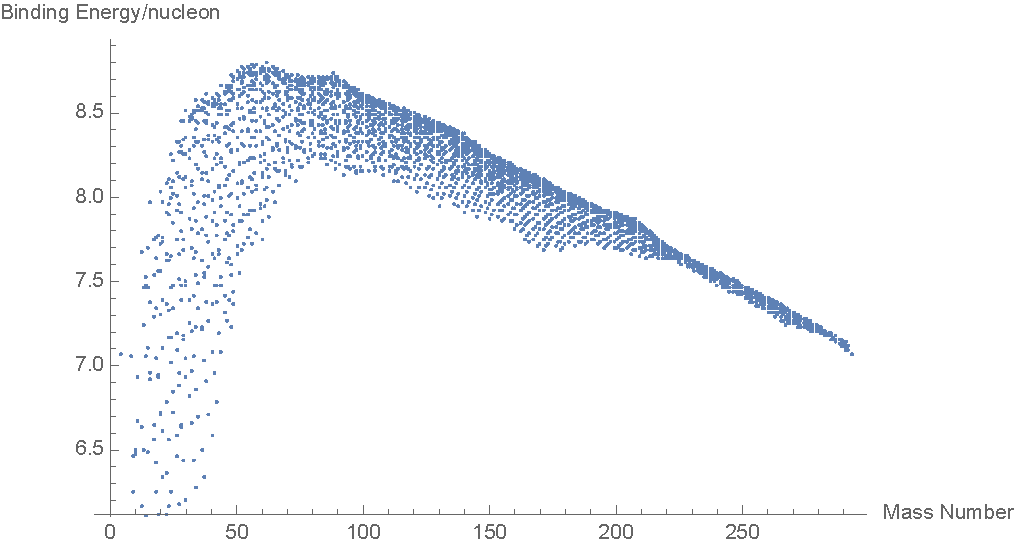
\includegraphics[width=0.8\textwidth]{isotopeChart}
  \end{enumerate}


\end{document}
